\documentclass[11pt]{article}

\usepackage{amsmath}
\usepackage{amssymb}
\usepackage{fancyhdr}
\usepackage{comment}
\usepackage{color}
\usepackage{graphicx}
\usepackage{listings}
\usepackage[colorlinks=true,linkcolor=blue,urlcolor=blue]{hyperref}

\newcounter{marks}
\def\maxmarks#1{\extramark{#1}\addtocounter{marks}{#1}}
\def\extramark#1{
  \begin{flushright}
  [\emph{#1 points}]
  \end{flushright}
%  \quad\mbox{\LARGE\begin{tabular}{|c|c|}
%  \hline\rule{1cm}{0cm} & #1 \\ \hline \end{tabular}}
}
\def\dumptotal{%
\begin{flushright}
\begin{tabular}{|l|} \hline
\LARGE{\textbf{\rule{0pt}{16pt}Total:~\themarks}} \\ \hline
\end{tabular}
\end{flushright}}
\def\skiplines#1{\newline \forloop{#1}{{\rule{0pt}{20pt}} \\}}

\specialcomment{answer}{\color{blue}}{\color{black}}
\def\withanswers{\def\skiplines##1{\relax}\def\skippage{\relax}}
\def\withoutanswers{\excludecomment{answer}\def\skippage{\clearpage}}

\newif\ifprint
\printtrue

\oddsidemargin0cm
\topmargin-2cm     %I recommend adding these three lines to increase the 
\textwidth16.5cm   %amount of usable space on the page (and save trees)
\textheight23.5cm  

\newcommand{\mycoursenum}{10-601}
\newcommand{\myhwnum}{2}
\newcommand{\myname}{Dawei}
\newcommand{\myandrew}{daweiwan}
\newcommand{\myfirstta}{Siddhartha Jain}
\newcommand{\mysecondta}{Ying Yang}

\newcommand{\question}[2] {\vspace{.25in} \hrule\vspace{0.5em} \noindent{\bf #1: #2} \vspace{0.5em} \hrule \vspace{.10in}}
\renewcommand{\part}[1] {\vspace{.10in} {\bf (#1)}}

\setlength{\parindent}{0pt}
\setlength{\parskip}{5pt plus 1pt}
 
\pagestyle{fancyplain}
\lhead{\fancyplain{}{\textbf{HW\myhwnum}}}
\ifprint
\rhead{\fancyplain{}{Andrew ID: \myandrew}}
\else
\rhead{\fancyplain{}{\myname\\ \myandrew}}
\fi
\chead{\fancyplain{}{\mycoursenum}}

\withoutanswers

\begin{document}

\medskip

\thispagestyle{plain}
\begin{center}
{\Large \mycoursenum: Homework \myhwnum} \\
Due: 25 September 2014 11:59pm (Autolab) \\
TAs: \myfirstta, \mysecondta \\
\medskip
\ifprint
Name: \myname \\
Andrew ID: \myandrew \\
\else
Name: \myname \\
Andrew ID: \myandrew \\
\fi
\end{center}

Please answer to the point, and do not spend time/space giving irrelevant details. 
%You should not require more space than is provided for each question. If you do, please think whether you can make your argument more pithy, an exercise that can often lead to more insight into the problem. 
Please state any additional assumptions you make while answering the questions. 
For Questions 1 to 5, 6(b) and 6(c), you need to submit your answers in a single PDF file on autolab, either a scanned handwritten version or a \LaTeX pdf file. 
Please make sure you write legibly for grading.
For Question 6(a), submit your m-files on autolab. 

You can work in groups. However, no written notes can be shared, or taken during group discussions. You may ask clarifying questions on Piazza. However, under no circumstances should you reveal any part of the answer publicly on Piazza or any other public website. The intention of this policy is to facilitate learning, not circumvent it. Any incidents of plagiarism will be handled in accordance with \href{http://www.cmu.edu/policies/documents/Academic%20Integrity.htm}{CMU's Policy on Academic Integrity}.


%%%%%%%%%%%%%%%%%%%%%%%%%%%%%%%%%%%%%%%%%%%
\question{$\star$}{Code of Conduct Declaration}

\begin{itemize}
	\item Did you receive any help whatsoever from anyone in solving this assignment? No.
	\item If you answered \emph{yes}, give full details: \rule{0.4\textwidth}{.4pt} (e.g. \emph{Jane explained to me what is asked in Question 3.4})
	\item Did you give any help whatsoever to anyone in solving this assignment? No.
	\item If you answered \emph{yes}, give full details: \rule{0.4\textwidth}{.4pt} (e.g. \emph{I pointed Joe to section 2.3 to help him with Question 2}).
\end{itemize}


\clearpage
%%%%%%%%%%%%%%%%%%%%%%%%%%%%%%%%%%%%%%%%%%%
\question{1}{A probabilistic view of linear regression. (TA:- \mysecondta)}
Let $X$ and $Y$  be two random variables,  $\beta$ be a constant vector, and $\epsilon \sim \mathcal{N}(0, \sigma^2)$ be a Gaussian random variable with zero mean and variance $\sigma^2$. 
We assume $Y = \beta X + \epsilon$, and that $\epsilon$ is independent of $X$.  \\

\part{a} Show that given $X = x$, the distribution of $Y$ is $\mathcal{N}(\beta x, \sigma^2)$
\maxmarks{3}

{\color{blue} Since $\beta$ is a constant scalar, and $x$ is an observed hence constant value, $\beta x$ is constant. 
That being said, we're deviating the original Gaussian distribution $N(0,\sigma^2)$ by an amount of $\beta x$, 
which yields $N(\beta x,\sigma^2)$ by common sense. That is, $Y\sim N(\beta x,\sigma^2)$. \hfill $\blacksquare$ }

\part{b} Let $\{(X_i, Y_i),i = 1, \cdots, n\}$ be $n$ independent samples from the model above. 
     Show that the maximum likelihood estimation of $\beta$, where the likelihood is with regard to the conditional distribution $Y|X$, is the least square solution
    \begin{align*}
    \hat\beta = \arg\min_{\beta}  \sum_{i=1}^{n} (Y_i - \beta X_i)^2
    \end{align*}
\maxmarks{3}

{\color{blue} In this case, the logarithmic likelihood function
\begin{align}
LL\left(Y_1|X_1,Y_2|X_2,\cdots,Y_n|X_n:\beta\right)=&\sum_{i=1}^n\ln f\left(Y_i|X_i:\beta\right) \\
=&\sum_{i=1}^n\ln\left[\frac1{\sigma\sqrt{2\pi}}\exp\left(-\frac{(Y_i-\beta X_i)^2}{2\sigma^2}\right)\right] \label{using-1a} \\
=&n\ln\frac1{\sigma\sqrt{2\pi}}-\frac1{2\sigma^2}\sum_{i=1}^n(Y_i-\beta X_i)^2 \label{1b-final}
\end{align}
which, reaches its maximum when $\sum_{i=1}^n(Y_i-\beta X_i)^2$ is at its minimum. \\
Therefore the maximum likelihood estimation $\beta$ is
\[\hat\beta = \arg\min_{\beta}  \sum_{i=1}^{n} (Y_i - \beta X_i)^2\]\hfill $\blacksquare$ }

\clearpage

%%%%%%%%%%%%%%%%%%%%%%%%%%%%%%%%%%%%%%%%%%%
\question{2}{One-dimensional ridge regression(TA:- \mysecondta)}

Let $Y$ and $X$ be two random variables, and $Y = \beta X + \epsilon$ given $X$, where $\beta$ is a constant, and $\epsilon \sim \mathcal{N}(0,\sigma^2)$, independent of $X$. 
Given $n$ independent sample pairs, $(x_1, y_1), (x_2, y_2), \cdots, (x_n, y_n)$,
instead of ordinary least square, here we estimate $\beta$ with ``ridge regression'', by solving the following problem. 
\begin{align*}
\hat{\beta} = \arg \min_{\beta}\frac{1}{2}\left(\sum_{i=1}^n(y_i- \beta x_i)^2 + \lambda \beta^2\right)
\end{align*}
where $\lambda \ge 0$ is a tuning parameter.\\ 

\part{a}Give a solution in explicit formula for $\hat \beta$.
\maxmarks{3}

{\color{blue}
We try to find an explicit solution by its partial differentiation:
\begin{align}
\frac{\partial}{\partial\beta}\frac{1}{2}\left(\sum_{i=1}^n(y_i- \beta x_i)^2 + \lambda \beta^2\right)
=&\frac{1}{2}\left(\sum_{i=1}^n2(y_i-\beta x_i)(-x_i) + 2\lambda \beta\right) \\
=&\sum_{i=1}^n(\lambda+x_i^2)\beta-\sum_{i=1}^n x_iy_i. \label{2a-final}
\end{align}
where we assume that $\lambda\beta^2$ is summed (it doesn't matter too much). Letting (\ref{2a-final}) be zero yields: 
\begin{equation}
	\hat \beta=\frac{\sum_{i=1}^n x_iy_i}{\sum_{i=1}^n(\lambda+x_i^2)}
\end{equation} \hfill$\blacksquare$} 

\part{b} When $\lambda$ goes from $0$ to infinity, how does $\hat \beta$ change? Give a brief explanation of your answer.
\maxmarks{2}

{\color{blue} $\hat\beta$ is a monotonically decreasing function with respect to $\lambda$. For $\lambda=0$, $\hat\beta$ devolves into 
the standard linear regression estimate; as $\lambda\rightarrow\infty$, $\beta\rightarrow0$, meaning that the
correlation between $X$ and $Y$ is getting weaker and weaker, and is finally diminished when $\lambda=\infty$. This is explained by 
the fact that the term that suggests a correlation, namely $(y_i-\beta x_i)^2$, is becoming trivial as $\lambda$ grows. \hfill$\blacksquare$ }


\clearpage
%%%%%%%%%%%%%%%%%%%%%%%%%%%%%%%%%%%%%%%%%%
\question{3} {Least square  (TA:- \mysecondta)}
 Suppose $X$ and $Y$ are random variables.  
     Let $(x_1, y_1),\cdots, (x_n,y_n)$  be $n$ pairs of samples. 
    Compute the least square solutions for the following models.
    $\epsilon \sim N(0, \sigma^2)$
    \begin{enumerate}
    \item $Y = \beta X + \epsilon$
    \item $Y = \beta^2 X + \epsilon$ 
    \end{enumerate}
    Which of the the models above yields to a lower training error?
    \maxmarks{5}
    
{\color{blue} The maximum likelihood estimate for the first model is known to be
\begin{equation}
	\hat\beta_1=\frac{\sum_{i=1}^nx_iy_i}{\sum_{i=1}^nx_i^2}
\end{equation}
However, we cannot directly assign $\hat\beta_2^2\leftarrow\hat\beta_1$ since $\hat\beta_1$ might be negative. Consider: 
\begin{equation}
	\hat\beta_2=\arg\min_{\beta}\sum_{i=1}^n\left(\beta^2x_i-y_i\right)^2
\end{equation}
To find the minimum points, we take its first and second order derivatives:
\begin{align}
	\frac{\partial}{\partial\beta}\sum_{i=1}^n\left(\beta^2x_i-y_i\right)^2&=
	\sum_{i=1}^n2\left(2\beta x_i\right)\left(\beta^2x_i-y_i\right)=4\beta^3\sum_{i=1}^nx_i^2-4\beta\sum_{i=1}^nx_iy_i \label{3-1d} \\
	\frac{\partial^2}{\partial^2\beta}\sum_{i=1}^n\left(\beta^2x_i-y_i\right)^2&=
	12\beta^2\sum_{i=1}^nx_i^2-4\sum_{i=1}^nx_iy_i
\end{align}
If $\sum_{i=1}^nx_iy_i\ge0$, we have two minimum points at $\pm\hat\beta_1^{0.5}$, and the second model will 
have the same performance as the first model, yielding the same training error; otherwise, 
the only minimum point would be $0$, and the second model will have worse performance, yielding 
a higher training error than the first model since it suggests no correlation between $X$ and $Y$ (i.e., not trained). 

Formally, the least square solution for the second model is:
\begin{equation}
	\hat\beta_2=\begin{cases}
		\pm\left[\dfrac{\sum_{i=1}^nx_iy_i}{\sum_{i=1}^nx_i^2}\right]^{0.5} & \sum_{i=1}^nx_iy_i>0 \\
		0 & \text{otherwise}
	\end{cases}	
\end{equation}
Intuitively 1. is always better than 2. since $\beta$ can be assigned with 
arbitrary real value, unlike $\beta^2$, which is limited to non-negatives.  \hfill $\blacksquare$}

\clearpage 
\question{4} {Behavior of linear regression (TA:- \myfirstta)}
 Suppose you know the number of keyboard and mice sold at various 
	locations around the world and from that you want to estimate the 
	number of computers sold using linear regression. Your model is $Y = 
	\beta_1 k + \beta_2 m$ where $Y$ is the number of computers sold, $k$ 
	is the number of keyboards sold and $m$ is the number of mice sold. You 
	get 101 observations such that 100 of them have 1 keyboard, 1 mouse and 
	1 computer, but the 101st has 1 keyboard, 0 mouse, and 1 computer.


For \part{a} and \part{b}, you can use \texttt{regress} in Matlab to compute the answers. \\
\part{a}
What are the optimal values of $\beta_1, \beta_2$ in the scenario above.
\maxmarks{3}	

{\color{blue} $\beta_1=1,\beta_2=0$. Computed with the following statements in Octave: \\
\texttt{> A = ones(101, 2); A(101, 2) = 0; y = ones(101, 1); \\ > P = inv(A'*A)*A'*y; }
\hfill$\blacksquare$
}

\part{b} Now suppose you get two additional observations, both with 0 keyboard, 1 mouse, and 1 computer. What are the optimal $\beta$ 
		values now?
\maxmarks{3}

{\color{blue} $\beta_1=0,\beta_2=1$. Computed with the following statements in Octave: \\
\texttt{> B = ones(103, 2); B(101, 2) = 0; B(102:103, 1) = 0; z = ones(103, 1); \\ > Q = inv(B'*B)*B'*z; } \hfill$\blacksquare$ }

\part{c} As you should notice, the optimal values for $\beta$ fluctuate 
wildly with the addition of even very few observations. This is a 
problem as then it's hard to converge on a set of values for $\beta$. 
Why is this behavior happening? Given an arbitrary dataset $X,Y$, how 
can we test whether such behavior might occur?

\maxmarks{3}

{\color{blue} Consider $k, m, y$ as the coordinates of a point in a 3-dimensional space, i.e., $P(k, m, y)$.
In the original dataset, there are 100 points stacking at $A(1, 1, 1)$, (almost) guaranteeing that the model output
would pass that particular point. However, there is no constraint on the line's orientation, such that any
point further supplied can be decisive on $\beta$. In (a), $\beta$ describes a line from $A$ to (1, 0, 1); In (b), 
$\beta$ describes a line from $A$ to $(0, 1, 1)$. It is expected, geometrically, that $\beta$ should be fluctuating
wildly with such {\it deliberately crafted} points. 

To test whether such behavior might occur, investigate whether there is a dense point cloud dwelling somewhere
in the joint observed input/output space. \hfill$\blacksquare$}

%%%%%%%%%%%%%%%%%%%%%%%%%%%%%%%%%%%%%%%%%%%


\clearpage
%%%%%%%%%%%%%%%%%%%%%%%%%%%%%%%%%%%%%%%%%%%
\question{5}{Gaussian Naive Bayes. (TA:- \mysecondta)}
Let $Y \in \{0,1\}$ be class labels,
and let $X \in \mathbb{R}^{p}$ denote a $p$-dimensional feature.\\  
\part{a}
In a Gaussian naive Bayes model, where the conditional distribution of each feature is a one-dimensional Gaussian, give a maximum-likelihood estimate (MLE) of the conditional distribution of feature $X^{(j)}, j = 1, \cdots, p$, ($X^{(j)} |Y \sim N(\mu^{(j)}_Y, (\sigma^{(j)}_Y)^2)$)
\maxmarks{4}

{\color{blue} Here we need to estimate the mean and variance for each individual feature:
\begin{equation}
	\ln L\left(X^j|Y;\mu_Y,\sigma_Y^2\right)=k_Y\ln\frac1{\sigma_Y^{(j)}\sqrt{2\pi}}-\frac1{2(\sigma_Y^{(j)})^2}\sum_{\Omega}\left(X^{(j)}_Y-\mu^{(j)}_Y\right)^2
\end{equation}
where the sum is performed over all data points labeled as class $Y$. Letting the derivatives be zero, 
\begin{align}
	\frac{\partial\ln L}{\partial\mu^{(j)}_Y}&=\frac1{(\sigma_Y^{(j)})^2}\left[-k_Y\mu_Y^{(j)}+\sum_{\Omega} x_Y^{(j)}\right]=0 \\
	\frac{\partial\ln L}{\partial(\sigma^{(j)}_Y)^2}&=-\frac12k_Y\frac{2\cdot2\pi}{2\pi(\sigma_Y^{(j)})^2}+\frac12\frac1{(\sigma_Y^{(j)})^4}
	\sum_{\Omega}\left(X^{(j)}_Y-\hat\mu^{(j)}_Y\right)^2=0
\end{align}
we can obtain a maximum likelihood estimate: \hfill$\blacksquare$ 
\begin{equation}
	\hat\mu_Y^{(j)}=\frac1{k_Y}\sum_{\Omega} x_Y^{(j)}
	\quad(\sigma_Y^{(j)})^2=\frac1{k_Y}\sum_{\Omega}\left(X^{(j)}_Y-\mu^{(j)}_Y\right)^2
\end{equation} }

 \part{b} 
In a full Gaussian Bayes model, we assume  that the conditional distribution 
$\Pr(X|Y)$ is a multidimensional Gaussian,  $X|Y \sim \mathcal{N}(\mu_Y, \Sigma_Y)$, where $\mu$ is the mean vector and $\Sigma \in \mathbb{R}^{p\times p}$ is the covariance matrix.  
Suppose the prior of $Y$ is already given.
How many parameters do you need to estimate in Gaussian naive Bayes model? How many in a full Gaussian Bayes model? 
\maxmarks{3}

{\color{blue} In the naive Bayes model, we need $2p$ parameters, with $p$ for the mean vector $\mu$, and the rest 
for the diagonal elements in $\Sigma$. In the full model, we need $0.5p(p+1)+p$ parameters, where $p$ comes
from the mean vector, and $0.5p(p+1)$ comes from the covariance matrix, since it's symmetric. \hfill$\blacksquare$ }
    
\part{c} In a two dimensional case, we can visualize how Naive Bayes behaves when input features are correlated.  
    A data set shown in Figure~\ref{fig:GNB} (A), 
    where red points are in Class 0, blue points are in Class 1.  
	The conditional distributions are two-dimensional Gaussians. 
	In (B) (C) and (D), the ellipses represent conditional distributions for each class. 
	The centers of ellipses show the mean and the contours show the boundary of two standard deviations. 	
	Which of them is most likely to be the true conditional distribution?
	Which of them is most likely to be estimates by a Gaussian naive Bayes model?
	If we assume the prior probabilities for both classes are equal, 
	which model will achieve a higher accuracy on the training data? \maxmarks{3}

{\color{blue} (C) is most likely to be the true conditional distribution. (B) is most likely
to be estimates of a Gaussian naive Bayes model. The full Gaussian model always has equal 
or better performance than the naive Bayes one since it has additional degrees of freedom. \hfill$\blacksquare$ }

\begin{figure}[h]
\begin{tabular}{cc}
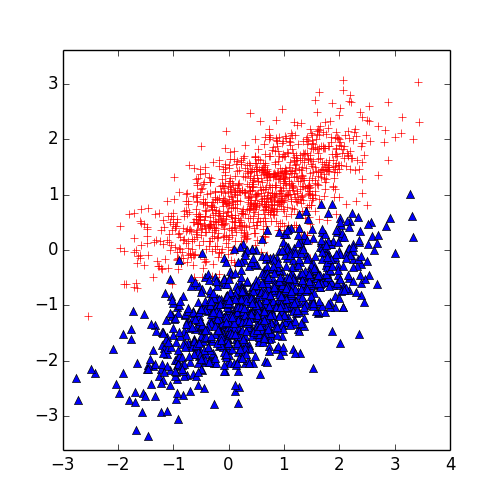
\includegraphics[width = 0.48\textwidth]{GNB_data.png}& 
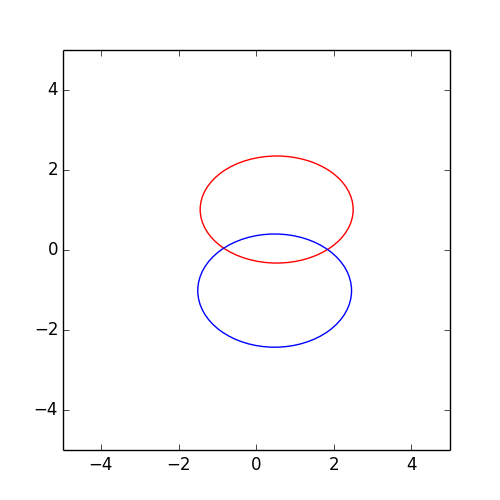
\includegraphics[width = 0.48\textwidth]{GNB_A.png}  \\
\text{ (A) Data} &  \text{ (B) } \\
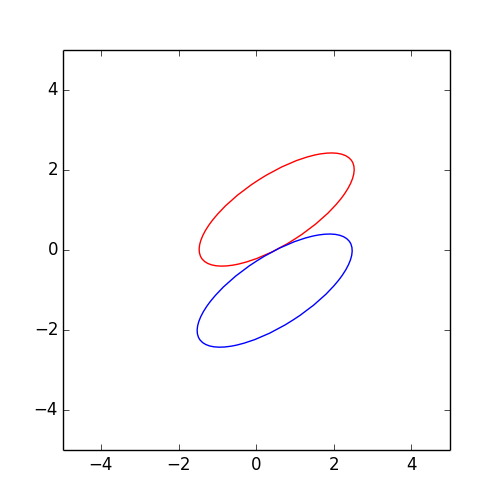
\includegraphics[width = 0.48\textwidth]{GNB_B.png} &
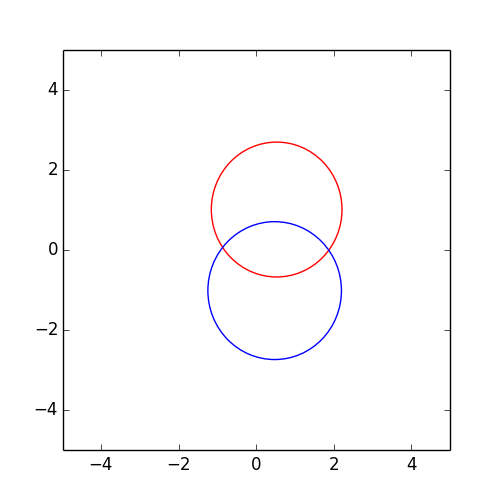
\includegraphics[width = 0.48\textwidth]{GNB_C.png} \\
\text{ (C)} &\text{(D)} \\
\end{tabular}
\caption{Figure of Q6 (c)}\label{fig:GNB}
\end{figure}


\clearpage

\question{6}{Text classification using Naive Bayes. (TA:- \myfirstta \& \mysecondta)}
In this assignment, you are going to program a naive Bayes classifier to classify documents from a serious European magazine ``economist'' (Class 1) and  a not-so-serious American megazine ``the onion'' (Class 0). \\
\begin{enumerate}

\item \textbf{Data description}\\
All data files are in \texttt{Onion\_vs\_Economist}.  
If you load the \texttt{handout.mat} into Octave (or Matlab) with
\texttt{load ’handout.mat’}, you will see the following matrices, 
\texttt{Xtrain,  Ytrain,  Xtest, Ytest}.
We also provided a dictionary of $V$ tokens (or words) in \texttt{dictionary.mat}, and denote the tokens in the dictionary by indices, $\{ 1,2, \cdots, V \}$.
There are $n$ training documents and $m$ testing documents. 
For each document, we counted the number of occurrence of each token, resulting in a vector $(c_1, c_2, \cdots, c_V)$. 
Each row in \texttt{Xtrain}  and \texttt{Xtrain} is such a vector for one document. 
\texttt{Ytrain} and \texttt{Ytest} are $n\times 1$ and $m\times 1$ 
binary class labels.

\iffalse
\item \textbf{Model description (Binomial model)}\\
Given a document in one class with label $Y=y$, we assume a binomial distribution for each word. 
For the $i$th word in the dictionary, $W_i = 1$ denotes that the word $i$ is present in the document, where as $W_i = 0$ denotes that the word $i$ is absent.  

With a naive Bayes model, we assume that the $V$ words are independent given the class label. 
Therefore the posterior probability is 
\begin{align*}
\Pr(Y = y |W_1, \cdots, W_q) \propto \prod_{i=1}^{V} \Pr( W_i| Y = y) \Pr( Y = y)
\end{align*}
Without smoothing,
\begin{align*} 
\Pr( W_i = 1 | Y = y) = \frac{  \text{ number of documents where the $i$th word is present in Class y }} { \text{ number of documents in Class y}} 
\end{align*}
You need to use additive smoothing
http://en.wikipedia.org/wiki/Additive\_smoothing in your implementation. \\
In addition, to avoid multiplying very small probabilities and underflow, you should use a logarithmic transformation to determine the predicted class label. 

\begin{align*}
 y^* & = \arg\max_y \Pr(Y = y |W_1, \cdots, W_V)  \\
     & =  \arg\max_y  \prod_{i=1}^{V} \Pr( W_i| Y = y) \Pr( Y = y)\\
     & =  \arg\max_y  (\sum_{i=1}^{V} \log \Pr( W_i| Y = y) + \log \Pr( Y = y)))
\end{align*}
\fi

\item \textbf{Model description (multinomial model)}\\
We view a document as an ordered sequence of word events. 
Suppose we have a document with label $Y=y \in \{0,1\}$, which contains $q$ words in total, we use the event $W_i = j$ to denote the event that the $i$th word is the $j$th token in the dictionary, $j \in \{ 1,2, \cdots, V \}$. 
With a naive Bayes model, we assume that the $q$ word events are independent, and have an identical multinomial distribution with $V$ outcomes. 

\textbf{Learning the conditional probability}\\
Given one training document in Class $y$, if we do not use smoothing ( or pseudocounts ), we estimate the conditional probability for a word event $W$ in the following way,
\begin{align*}
\Pr( W = j| Y = y)  &= \frac{ \text{ number of occurance of token $j$}}{ \text{ total number of words }} \\
&  = \frac{ \text{ number of occurance of token $j$}}{ \text{ total number of occurance of all $V$ tokens  }}
\end{align*}
In \texttt{Xtrain}, you are given multiple training documents in one class, you should think in a way as concatenating them all into a large document. 
You need to use additive smoothing (or pseudocount)
http://en.wikipedia.org/wiki/Additive\_smoothing in your implementation, setting $\alpha = 1$. \\

\textbf{Learning the prior}\\
Assume the prior distribution of label $Y$ is binomial, without smoothing, it is estimated as 
\[ \Pr(Y = y) = \frac{ \text{number documents in Class y}} { \text{total number of documents}}\] 


\textbf{Making prediction}\\
Now given the test document of length $q$, 
\begin{align*}
y* &= \arg\max_y \Pr(Y = y |W_1, \cdots, W_q)  = \arg\max_y \frac{ \prod_{i=1}^{q} \Pr( W_i| Y = y) \Pr( Y = y)}{ \Pr (W_1, \cdots, W_q)} \\
& = \arg\max_y (\prod_{i=1}^{q} \Pr( W_i| Y = y) \Pr( Y = y)) 
\end{align*}
However, we are only given the word counts of the document, $(c_1, c_2, \cdots, c_V)$,  and we can only compute the multinomial probability.
\begin{align}
y* &= \arg\max_y (  q! \prod_{j = 1}^{V} \frac{\Pr(W = j| Y=y)} {c_j!} \Pr( Y = y) \\ 
   & = \arg\max_y (\sum_{i=1}^{V} \log \Pr(W = j| Y=y) + \log \Pr(Y= y)) + \log (q!) - \sum_{i=1}^{V}\log(c_j!) \\ 
   & = \arg\max_y (\sum_{i=1}^{V} \log \Pr(W = j| Y=y) + \log \Pr(Y= y)) + \text{constant} \label{eq:log}
\end{align}
In your implementation, to avoid multiplying very small probabilities 
and underflow, you should use the logarithmic transformation 
as in Equation~\ref{eq:log}. 
\end{enumerate}
 
For \part{a}  submit your m-files to autolab. 
For \part{b} and \part{c}, write your solutions in your pdf. 


\part{a} Create following three octave functions and save them in three 
files, \texttt{nb\_train.m}, \texttt{nb\_test.m} and \texttt{nb\_run.m}.
\begin{verbatim}
model = nb_train(Xtrain, Y_train)
Pred_nb = nb_test(model, Xtest)
accuracy = nb_run(Xtrain, Ytrain, Xtest, Ytest)
\end{verbatim}
\texttt{model} is a structure that describe the model you learned. 
\texttt{Pred\_nb} is a $m\times 1$ binary vector, which denotes your prediction for the testing documents. 
In \texttt{nb\_run}, return the prediction accuracy  computed by \texttt{accuracy = mean(Pred\_nb==Ytest)} , and use \texttt{save('Pred\_nb.mat','Pred\_nb')} to save your prediction into a 
mat file. \\

\textbf{Note:} Your score will be determined by your classification 
accuracy on the test dataset you've been given as well as the held-out 
dataset that has not been released.

\lstset{
  numbers = left,
  language = Octave,
  basicstyle = \small,
  keywordstyle = \bfseries,  
}

{\color{blue} The functions are quite short. I just pasted them here for completeness.
\begin{lstlisting}
function model = nb_train(x, y)
  cumcount = [!y'*x; y'*x]; % concatenate & count; 
  model.prior = [!y'*!y; y'*y] / rows(y); % compute priors; 
  model.condpr = bsxfun(@rdivide, cumcount + 1, sum(cumcount, 2) + columns(x));
endfunction
\end{lstlisting}
\begin{lstlisting}
function Pred_nb = nb_test(model, x)
  likelihood = bsxfun(@plus, log(model.condpr)*x', model.prior);
  Pred_nb = diff(likelihood)' > 0;
endfunction
\end{lstlisting}
\begin{lstlisting}
function accuracy = nb_run(Xtrain, Ytrain, Xtest, Ytest)
  model = nb_train(Xtrain, Ytrain);
  Pred_nb = nb_test(model, Xtest);
  accuracy = mean(Pred_nb == Ytest);
  save('Pred_nb.mat', 'Pred_nb');
endfunction
\end{lstlisting}
}

\maxmarks{15}
\part{b} For the $j$th token in the dictionary, we can compute the following log-ratio,
\[
\left |\log \frac{Pr(W = j | Y = 1) }{Pr(W = j | Y = 0)} \right|
\]
Use this log-ratio as a measure, find the top five words that are most 
discriminative of the classes, report them in your pdf. 
\maxmarks{5} 

{\color{blue} This can be done by typing the following commands (provided that files are loaded):
\begin{lstlisting}
model = nb_train(Xtrain, Ytrain, Xtest, Ytest); 
[~, idx] = sort(abs(diff(log(model.condpr))), "descend");
dict(idx(1: 5)); 
\end{lstlisting} 
and the most discriminative words are: {\it percent}, {\it monday}, {\it yankees}, {\it sox}, {\it schmuck}. {\hfill$\blacksquare$}}

\part{c}  State the Naive Bayes assumption. 
Are there any pairs of words that violate the Naive Bayes assumption? 
If so, give 1 example of such pairs and explain why they might be 
violating the Naive Bayes assumption. 
\maxmarks{5}

{\color{blue} Naive Bayes: Given the class label, the presence of words are conditionally mutually independent. 
It would be impossible to proof or refute the dependence among any pair of words based on finite number of 
observations. But in this problem's scenario per se, it might be feasible to find some by common sense. 
For example, {\it the} and {\it onion} could be one; or {\it the} and {\it economist}, since they're known 
to be appearing together. {\hfill$\blacksquare$} }


\dumptotal

\end{document}

